\section{Is ground-truth-free selection predictable?}
\label{sec:selection}

\paragraph{Model.}
Fix an image and a solver.
Each run is independently \good with probability $p$, a global or partial \orbit error with probabilities $o_g$ and $o_p$, \cons with probability $c$, and \incons otherwise.
Let $q=p+o_g+o_p$ and $\kappa=q+c$, the probability of not being \incons.
This is not the pass probability $s$ of \cref{prop:stop}: with $\tau_S=\tau$, about $5\%$ of \good runs fail the threshold, and a label-free $\tau_S$ slightly above $\tau$ lets some \incons runs pass\claim{C-V5}.
We assume (S1) that \incons runs have a larger residual than all others.
We also assume (S3) that the orientation test fixes a global orbit error with probability $\phi_g$ and a partial one with probability $\phi_p$, and breaks a \good run with probability $h$.
The usual further assumption is (S2): within \good, \orbit and \cons, residual ranks are exchangeable.
Then, with $a=(1-h)p+\phi_go_g+\phi_po_p$,
\begin{equation}
\Oorb(K)=1-(1-q)^K,\quad \Eone(K)=\bigl[1-(1-\kappa)^K\bigr]\,a/\kappa,
\label{eq:curves}
\end{equation}
and similarly for $\Oraw$ and $\Eo$; each is the probability that the policy returns a \good image\claim{C-T5}.
This is the imperfect-verifier model of best-of-$n$~\cite{stroebl2026limits}.
\cons runs are its false positives, and orbit errors are false positives that no measurement-based verifier can reject (\cref{sec:setup}).
Its oracle gap never shrinks with $K$\claim{C-T6}.

Our data reject (S2).
Among the $100$ image--solver pairs whose passing runs mix a \good run with another class, $\Eo$ picks the \good run in $92$, against $51.9$ expected under (S2)\claim{C-A7}.
We therefore model the residual minimizer as the winner of a race with class weights $w$ (Plackett--Luce), fitted per solver to the within-image ranks of the first four runs.
This is the tail competition of best-of-$n$~\cite{yano2026tail}: a \cons run is picked only if it beats every \good run, not merely if it passes.
Relative to $w_G=1$, the weights $(w_O,w_C)$ of orbit errors, global or partial, and of \cons runs are $(0.17,0.020)$ for DAPS-2K, $(0.95,0.045)$ for SITCOM and $(0.037,0.024)$ for FAST-DIPS\claim{C-T11}.
Under the race, the per-image ceiling of $\Eo$ is $p/(p+(o_g+o_p)w_O+cw_C)$ rather than $p/\kappa$, and the oracle gap can peak and then shrink with $K$ (supplement)\claim{C-T10}.
Heterogeneity across images enters through a Dirichlet mixture over the class probabilities; it is the only dependence between the runs of an image.

\paragraph{Exact estimators.}
Averaging a policy over all $K$-subsets of an image's $n$ runs gives an unbiased, closed-form estimate: an argmin rule selects the run of residual rank $r$ with probability $\binom{n-r}{K-1}/\binom nK$, and success takes the pass@$k$ form $1-\binom{n-g}{K}/\binom nK$ for $g$ successful runs~\cite{chen2021codex}\claim{C-T7}.

\paragraph{Six prospective tests.}
For each test, we fitted the models to the runs already observed and registered forecasts with predictive intervals.
They cover (S2), the race, and two sensitivity variants of the race, one with a tighter prior on its log-weights (supplement).
Only then did we score the remaining runs (registry and hashes in the supplement)\claim{C-R1}\claim{C-R2}\claim{C-R3}.
\Cref{tab:forecasts} and \cref{fig:calib} compare the race with the exchangeable reference.
Over all six tests, the race's mean interval score~\cite{gneiting2007scoring} for the selected run is $30$ points and its mean absolute error $3.1$ points, against $182$ and $8.0$ for (S2); the race loses tests 1 and 4\claim{C-R8}.
Where wrong runs often fit the measurement (tests 2, 3, 5 and 6), the race's forecasts for the selected run cover all $55$ outcomes, and those of (S2) cover $3$.
On test 6, whose $100$ ImageNet images no earlier experiment had touched, the race covers all $10$ and (S2) none\claim{C-N3}.
Where wrong runs rarely fit the measurement (DAPS-2K, test 4), the two models nearly coincide\claim{C-R6}.

The forecasts fail on generation, \ie on whether any run is good.
They overestimate this coverage in five of six tests, including test 5, which was fitted to sixteen runs per image.
Between $16$ and $64$ runs, the share of ImageNet images with a \good run in some orientation rises only from $75\%$ to $78\%$, against $84$--$90\%$ forecast, and $22$ images never yield one\claim{C-R7}.
On ImageNet$'$ (test 6) it is $75\%$ at $64$ runs, against $88\%$ forecast, with $25$ images never solved.

\begin{table}[t]
\centering\footnotesize
\setlength{\tabcolsep}{2.2pt}
\begin{tabular}{@{}clccccc@{}}
\toprule
 & & Runs seen & \multicolumn{3}{c}{Selected run: covered (IS)} & Oracles \\
\cmidrule(lr){4-6}\cmidrule(l){7-7}
Test & Solver, data & $\to$ scored & & Race & (S2) & Race \\
\midrule
1 & FAST-DIPS, FF & $4\to64$ & & 9/42 (61) & 36/42 (11) & 10/42 \\
2 & FAST-DIPS, IN & $4\to16$ & & 9/9 (16) & 0/9 (398) & 3/6 \\
3 & SITCOM, FF & $4\to16$ & & 18/18 (12) & 2/18 (339) & 13/18 \\
4 & DAPS-2K, FF & $2$--$4\to8$ & & 12/14 (9) & 14/14 (8) & 9/14 \\
5 & FAST-DIPS, IN & $16\to64$ & & 18/18 (11) & 1/18 (264) & 2/12 \\
6 & FAST-DIPS, IN$'$ & $4\to64$ & & 10/10 (12) & 0/10 (516) & 3/10 \\
\midrule
All & & & & 76/111 (30) & 53/111 (182) & 40/102 \\
\bottomrule
\end{tabular}
\caption{\textbf{Registered forecasts against outcomes.} Forecasts whose $95\%$ predictive interval covers the outcome, for the selected run ($\Eo$, and $\Eone$ where registered) and for the oracles ($\Oraw$, $\Oorb$), over cohorts and $K$. IS: mean $95\%$ interval score in points, the interval width plus $40$ times any miss~\cite{gneiting2007scoring}; lower is better. Forecasts within a test are correlated across $K$, so the tests, not the forecasts, are the units of evidence. FF: FFHQ. IN: ImageNet. IN$'$: $100$ unseen images\claim{C-R8}\claim{C-F1}\claim{C-R4}\claim{C-R5}\claim{C-R6}\claim{C-R7}\claim{C-N3}.}
\label{tab:forecasts}
\end{table}

\paragraph{Selection was forecast well; generation was not.}
A retrospective diagnosis, which no forecaster could run, separates the two.
Given each FFHQ image's realized $64$ classes, the frozen race weights predict the observed $\Eo$ within $1.4$ points at every $K$, and those of the tighter-prior variant within $0.3$.
(S2) falls $4$--$7$ points short at every $K$.
Given also each run's realized orientation decision, the same holds for $\Eone$: the race is within $0.8$ points, and (S2) $2.5$--$4.7$ short (exploratory, with frozen parameters)\claim{C-F3}.
For SITCOM, the race is $1.5$--$2.8$ points high, and (S2) $12.8$ points low\claim{C-R5}.
By the frozen comparison rule, (S2) nevertheless covers more of test~1's selected-run outcomes ($36$ of $42$, against $9$).
Its pessimistic selection offsets the optimistic generation that all variants share\claim{C-F1}.
The generation miss has a simple anatomy.
Of the $25$ FFHQ images without a \good run among their first four, $18$ produced one later, and $7$ never did in $64$ runs, against $2.2$ forecast.
The mixture shrinks an image with four failures toward its cohort's success rate\claim{C-F2}.
Six of the seven never produced a measurement-consistent run\claim{C-F5}.
On ImageNet, $25$ of $100$ images have no \good run in any orientation among $16$\claim{C-R4}.

\paragraph{Why a few runs cannot see unsolved images.}
From class counts alone, four runs per image identify only the first four moments of the per-image mixture.
Two mixtures that agree on every four-run count can differ by $9.6$ points in $\Oraw$ at $K{=}64$\claim{C-T8}.
In our data, the four-run counts confine the population value of $\Oraw(64)$ for cohort~B only to $[0.611,1]$ (an outer enclosure; exploratory; supplement)\claim{C-B1}.
A few class counts cannot identify the mass near zero success, and $\textsc{flag}_C$ does not isolate it either (\cref{sec:protocol}); image features or residual trajectories might, which we did not test.

\begin{figure}[t]
\centering
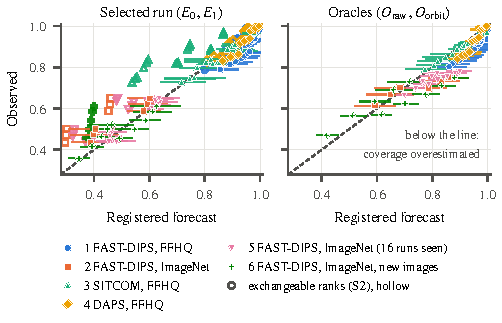
\includegraphics[width=\linewidth]{fig/forecast_calibration.pdf}
\caption{\textbf{Registered forecasts against outcomes, six prospective tests.} Each point is one cohort, $K$ and policy. Filled: the race model's forecast, with its $95\%$ predictive interval. Hollow: the exchangeable-ranks reference (S2). Left: the selected run. Right: the oracles, \ie whether any run is good; most points fall below the diagonal, where coverage was overestimated\claim{C-F1}\claim{C-R4}\claim{C-R5}\claim{C-R6}\claim{C-R7}.}
\label{fig:calib}
\end{figure}
